\documentclass[10pt,a4paper,twocolumn,twoside]{article}
\usepackage[utf8]{inputenc}
\usepackage[english]{babel}
\usepackage{multicol}
\usepackage{graphicx}
\usepackage{fancyhdr}
\usepackage{times}
\usepackage{titlesec}
\usepackage{multirow}
\usepackage{lettrine}
\usepackage[top=2cm, bottom=1.5cm, left=2cm, right=2cm]{geometry}
\usepackage[figurename=Fig.,tablename=TAULA]{caption}
\PassOptionsToPackage{hyphens}{url}\usepackage{hyperref}
\usepackage{listings}
\usepackage[htt]{hyphenat}
\usepackage{float}

\lstset{
  breaklines=true,
  tabsize=2,
}

\captionsetup[table]{textfont=sc}

\titlespacing*{\section}{0pt}{0.5cm}{0.2cm}
\titlespacing*{\subsection}{0pt}{0.5cm}{0.2cm}


\graphicspath{{img/}}

\author{\normalsize\sffamily Kevin Martín Fernández}
\title{\huge{\sffamily GEOSpectralSimulator: Multispectral terrain generator and viewer}}
\date{}

\newcommand\blfootnote[1]{%
  \begingroup
  \renewcommand\thefootnote{}\footnote{#1}%
  \addtocounter{footnote}{-1}%
  \endgroup
}

%No ident
\setlength\parindent{0pt}

%
%\large\bfseries\sffamily
\titleformat{\section}
{\large\sffamily\scshape\bfseries}
{\textbf{\thesection}}{1em}{}

%List counter enumerate
\renewcommand{\labelenumii}{\theenumii}
\renewcommand{\theenumii}{\theenumi.\arabic{enumii}.}
\renewcommand{\labelenumiii}{\theenumiii}
\renewcommand{\theenumiii}{\theenumii \arabic{enumiii}.}

\begin{document}

\fancyhead[LO]{\scriptsize Kevin Martín - GEOSpectralSimulator: Multispectral terrain generator and viewer}
\fancyhead[RO]{\thepage}
\fancyhead[LE]{\thepage}
\fancyhead[RE]{\scriptsize EE/UAB TFG INFORMÀTICA - GEOSpectralSimulator: Multispectral terrain generator and viewer}

\fancyfoot[CO,CE]{}

\fancypagestyle{primerapagina}
{
   \fancyhf{}
   \fancyhead[L]{\scriptsize TFG EN ENGINYERIA INFORMÀTICA, ESCOLA D'ENGINYERIA (EE), UNIVERSITAT AUTÒNOMA DE BARCELONA (UAB)}
   \fancyfoot[C]{\scriptsize June 2019. Escola d'Enginyeria (UAB)}
}

%\lhead{\thepage}
%\chead{}
%\rhead{\tiny EE/UAB TFG INFORMÀTICA: TÍTOL (ABREUJAT SI ÉS MOLT LLARG)}
%\lhead{ EE/UAB \thepage}
%\lfoot{}
%\cfoot{\tiny{February 2015, Escola d'Enginyeria (UAB)}}
%\rfoot{}
\renewcommand{\headrulewidth}{0pt}
\renewcommand{\footrulewidth}{0pt}
\pagestyle{fancy}

%\thispagestyle{myheadings}
\twocolumn[\begin{@twocolumnfalse}

{
\vspace*{-1cm}
\maketitle
}

\thispagestyle{primerapagina}
%\twocolumn[\begin{@twocolumnfalse}
%\maketitle
%\begin{abstract}
\begin{center}
\parbox{0.915\textwidth}
{\sffamily\small
\textbf{Resum--} En aquest projecte es pot veure com a partir de dades de satèl·lit es generen escenaris 3D que poden ser llegits en motors gràfics. Aquests objectes se'ls associa informació geogràfica en fitxers JSON que permeten a un simulador desenvolupat en Unreal Engine llegir-los, carregar les textures i situar-se en aquella posició del món físic utilitzant coordenades UTM. Això permet generar trajectòries on es prendran mostres amb les càmeres simulades. Les fonts de dades poden ser de diversos tipus destacant aquelles de tipus multispectral, aquestes seqüències d'imatges serviran per generar datasets per l'entrenament d'algorismes de deep learning.
\\
\\
\textbf{Paraules clau-- }
Simulador, Terreny, Satèl·lit, Multispectral, Unreal Engine\\
\\
\textbf{Abstract--}  In this project you can see how satellite data generates 3D scenarios that can be read in graphic engines. These objects are associated with geographic information in JSON files that allow a simulator developed in Unreal Engine to read them, load textures and position themselves in that position of the physical world using UTM coordinates. This allows you to generate trajectories where samples will be taken with the simulated cameras. The data sources can be of several types emphasizing those of multispectral type, these sequences of images will serve to generate datasets for the training of algorithms of deep learning.
\\
\\
\textbf{Keywords-- }
Simulator, Terrain, Satellite, Multispectral, Unreal Engine\\
\\
%\end{abstract}
}

\bigskip

{\vrule depth 0pt height 0.5pt width 4cm\hspace{7.5pt}%
\raisebox{-3.5pt}{\fontfamily{pzd}\fontencoding{U}\fontseries{m}\fontshape{n}\fontsize{11}{12}\selectfont\char70}%
\hspace{7.5pt}\vrule depth 0pt height 0.5pt width 4cm\relax}

\end{center}

\bigskip
%\end{abstract}
\end{@twocolumnfalse}]

\blfootnote{$\bullet$ E-mail de contacte: kevinmf94@gmail.com}
\blfootnote{$\bullet$ Menció realitzada: Enginyeria de Computació}
\blfootnote{$\bullet$ Treball tutoritzat per: Felipe Lumbreras Ruíz}
\blfootnote{$\bullet$ Curs 2018/19}

\vspace{-1cm}
\section{Introduction}
The simulation of real worlds for the generation of synthetic images is a field of high impact with the new resurgence of deep learning as a possible source of data. In this field we want to represent the real world as accurately as possible, thanks to this we can generate unlikely situations necessary for learning. This need is required when you want to represent real environments that may present a danger. For example, situations of risk (earthquakes, floods, fires, etc.), which have an economic impact (agriculture, resources, infrastructure, etc.) or others. (natural environment, people, etc.).
\\
\\
In this project, the information is generated by elevation maps and aerial images of real terrains. This data is used to create a simulated environment that can generate new data sets. This will generate data that can be used in multiple areas of computer learning. In addition, this project can simulate flights, see a geographic area or expand to other fields that use geographic information. This geographic information can be obtained from multiple sources (satellite data, aerial images, unmanned aircraft captures, virtual generated data, etc.), which allows to work with a large amount of external data.

\section{Objectives}

The main objective of this project is to create a tool to download geographic data and transform it into a 3D representation. In order to carry it out the following subobjectives must be completed: visualize the representation in a 3D engine, visualize multispectral data, move through the terrain (know the UTM position in the world), control a virtual vehicle through an external script or keyboard, generate a set of data that can be used in other algorithms, etc. The complete list can be seen in the appendix \ref{appendix:objectives}.

\section{Methodology}
In this project an Agile methodology is used. This allows us to identify more efficiently the small parts that make up the project and adapt them to the necessary changes. More specifically, a technique called Kanban \cite{kanban} is used. Kanban consists of organizing the backlog (list of short-term tasks) in cards that will be placed on a board according to the state of the task (To-Do, Doing, Done). For this purpose, Trello \cite{trello} is used, a software that allows to see the boards in a web browser, create cards and move them between different lists.
\\
A Gantt chart has been included to manage the project. In this diagram, several tasks and subtasks are taken into account to make a prediction of the work done, what remains to be done and the approximate time each task will take. This allows us to plan the project with a precise use of time.

\section{State of the art}
\label{estatart}

Currently, there are several solutions for the generation of images in simulated environments. Some of these simulations are used to generate the data used in machine learning algorithms. On the other hand, there are many sources where to take the initial data (geographical and topographic information) for these simulations.

In this field, some of the most important tools are AirSim \cite{airsim} developed by Microsoft and Carla SIMULATOR \cite{carla} developed by ``Centre de Visio per Computador (CVC)'', and others, like LESS \cite{less}, DIRSIG \cite{dirsig} or Google Earth Engine \cite{googleearth} for more specific scopes.

\subsection{AirSim}
AirSim is a graphic simulator made with Unreal Engine. This simulator has the purpose of generating synthetic images in simulated environments. AirSim incorporates multiple modules that offer the following features (Figure \ref{fig-airsim} shows an example): car simulation, drone simulation, real drone driver compatibility, recording, depth view, segmentation view, rain effects, lighting control according to the time of day, vehicle control through a python script, etc.

\begin{figure}[h]
\centering
  	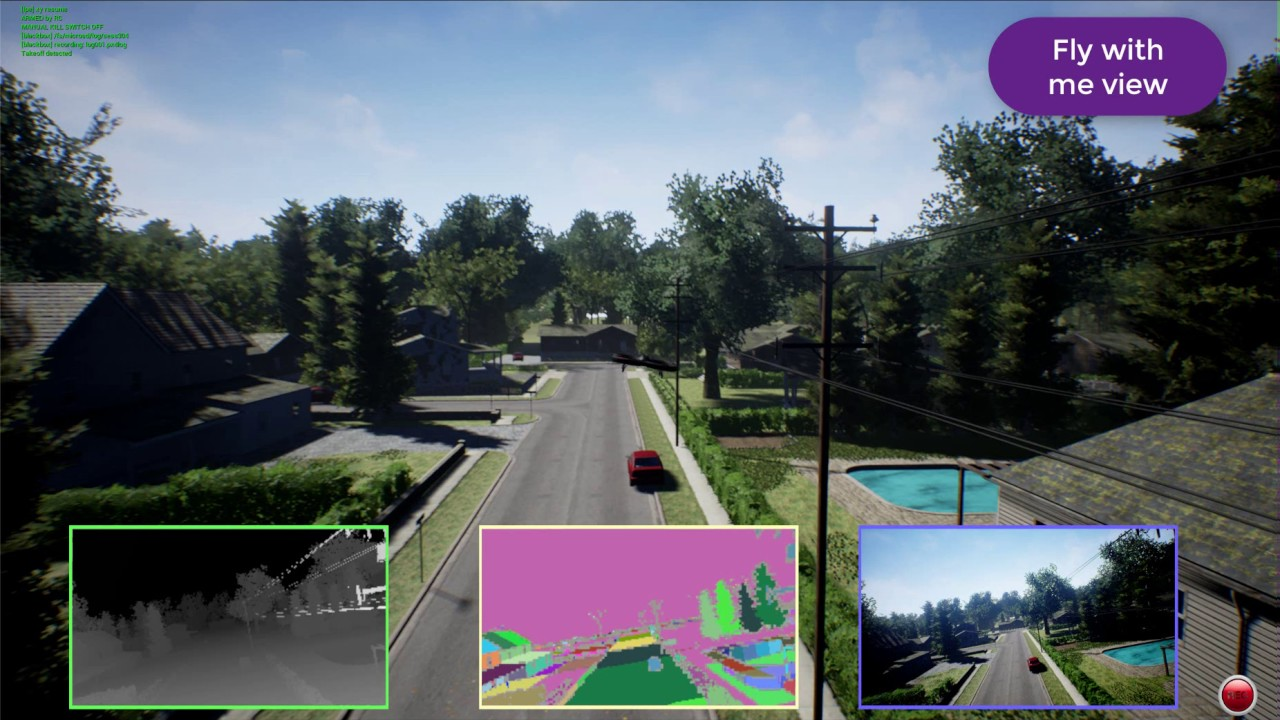
\includegraphics[width=0.49\textwidth]{airsim}
	\caption{Snapshot of AirSim simulator.}
	\label{fig-airsim}
\end{figure}

\subsection{Carla SIMULATOR}

Carla is a graphic simulator made with Unreal Engine, this simulator has the purpose of generating images in a simulated environment with the maximum realism to generate images. These images are used in neural networks to safely drive an autonomous car. Thanks to the simulated environment it is possible to take into account the unlikely cases that are difficult to generate in the real world (Figure \ref{fig-carla} shows a view of a scenario). Carla has the following characteristics: car simulation, in-depth view, segmentation view, traffic simulation, simulation of pedestrians, control of the actors (traffic, pedestrians, cameras, etc.) with a python script, etc.

\begin{figure}[h]
\centering
  	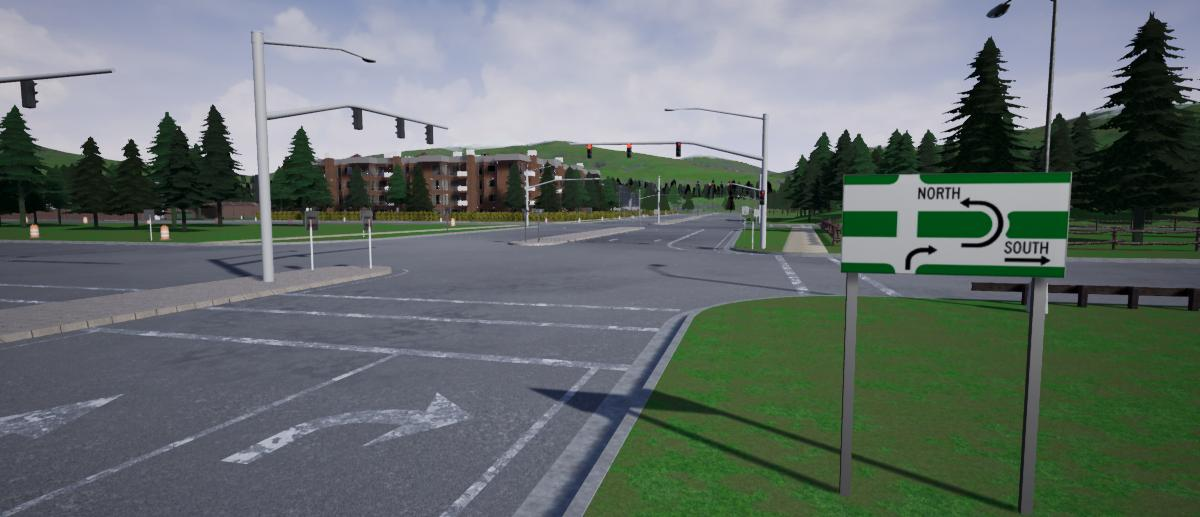
\includegraphics[width=0.49\textwidth]{carlatown}
	\caption{Carla example scene.}
	\label{fig-carla}
\end{figure}

\subsection{LESS}

LESS represents a radiation model (Figure \ref{fig-lessradiacio} shows an example) generated in a three-dimensional object/terrain for different rays. It is generated from a ray tracing technique, this allows to simulate data and images on realistic three-dimensional scenes. This model implements a weighted photon tracking method to simulate the effect of bidirectional multispectral reflectance.

\begin{figure}[h]
\centering
  	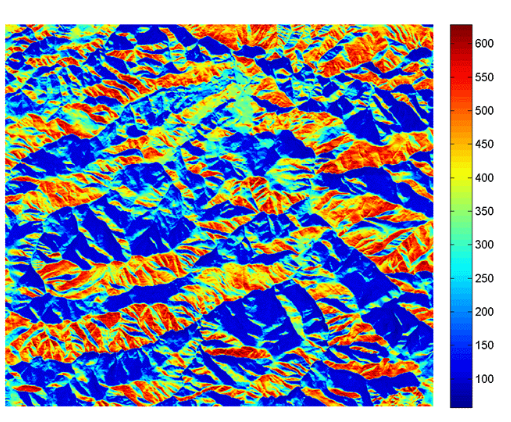
\includegraphics[width=0.4\textwidth]{lessradiacio}
	\caption{Example of results of the radiation of a terrain.}
	\label{fig-lessradiacio}
\end{figure}

\subsection{DIRSIG}
The model of Digital Imaging and Remote Sensing Image Generation (DIRSIG) is a model of generation of synthetic images developed by the lab of Digital Imaging and Remote Sensing of the Rochester Institute of Technology. The model can produce one band, multispectral or hyperspectral images from the visible to the infrared region of the electromagnetic spectre. You can see an example generated by DIRSIG on the figure \ref{fig-tacoma}.

\begin{figure}[h]
\centering
  	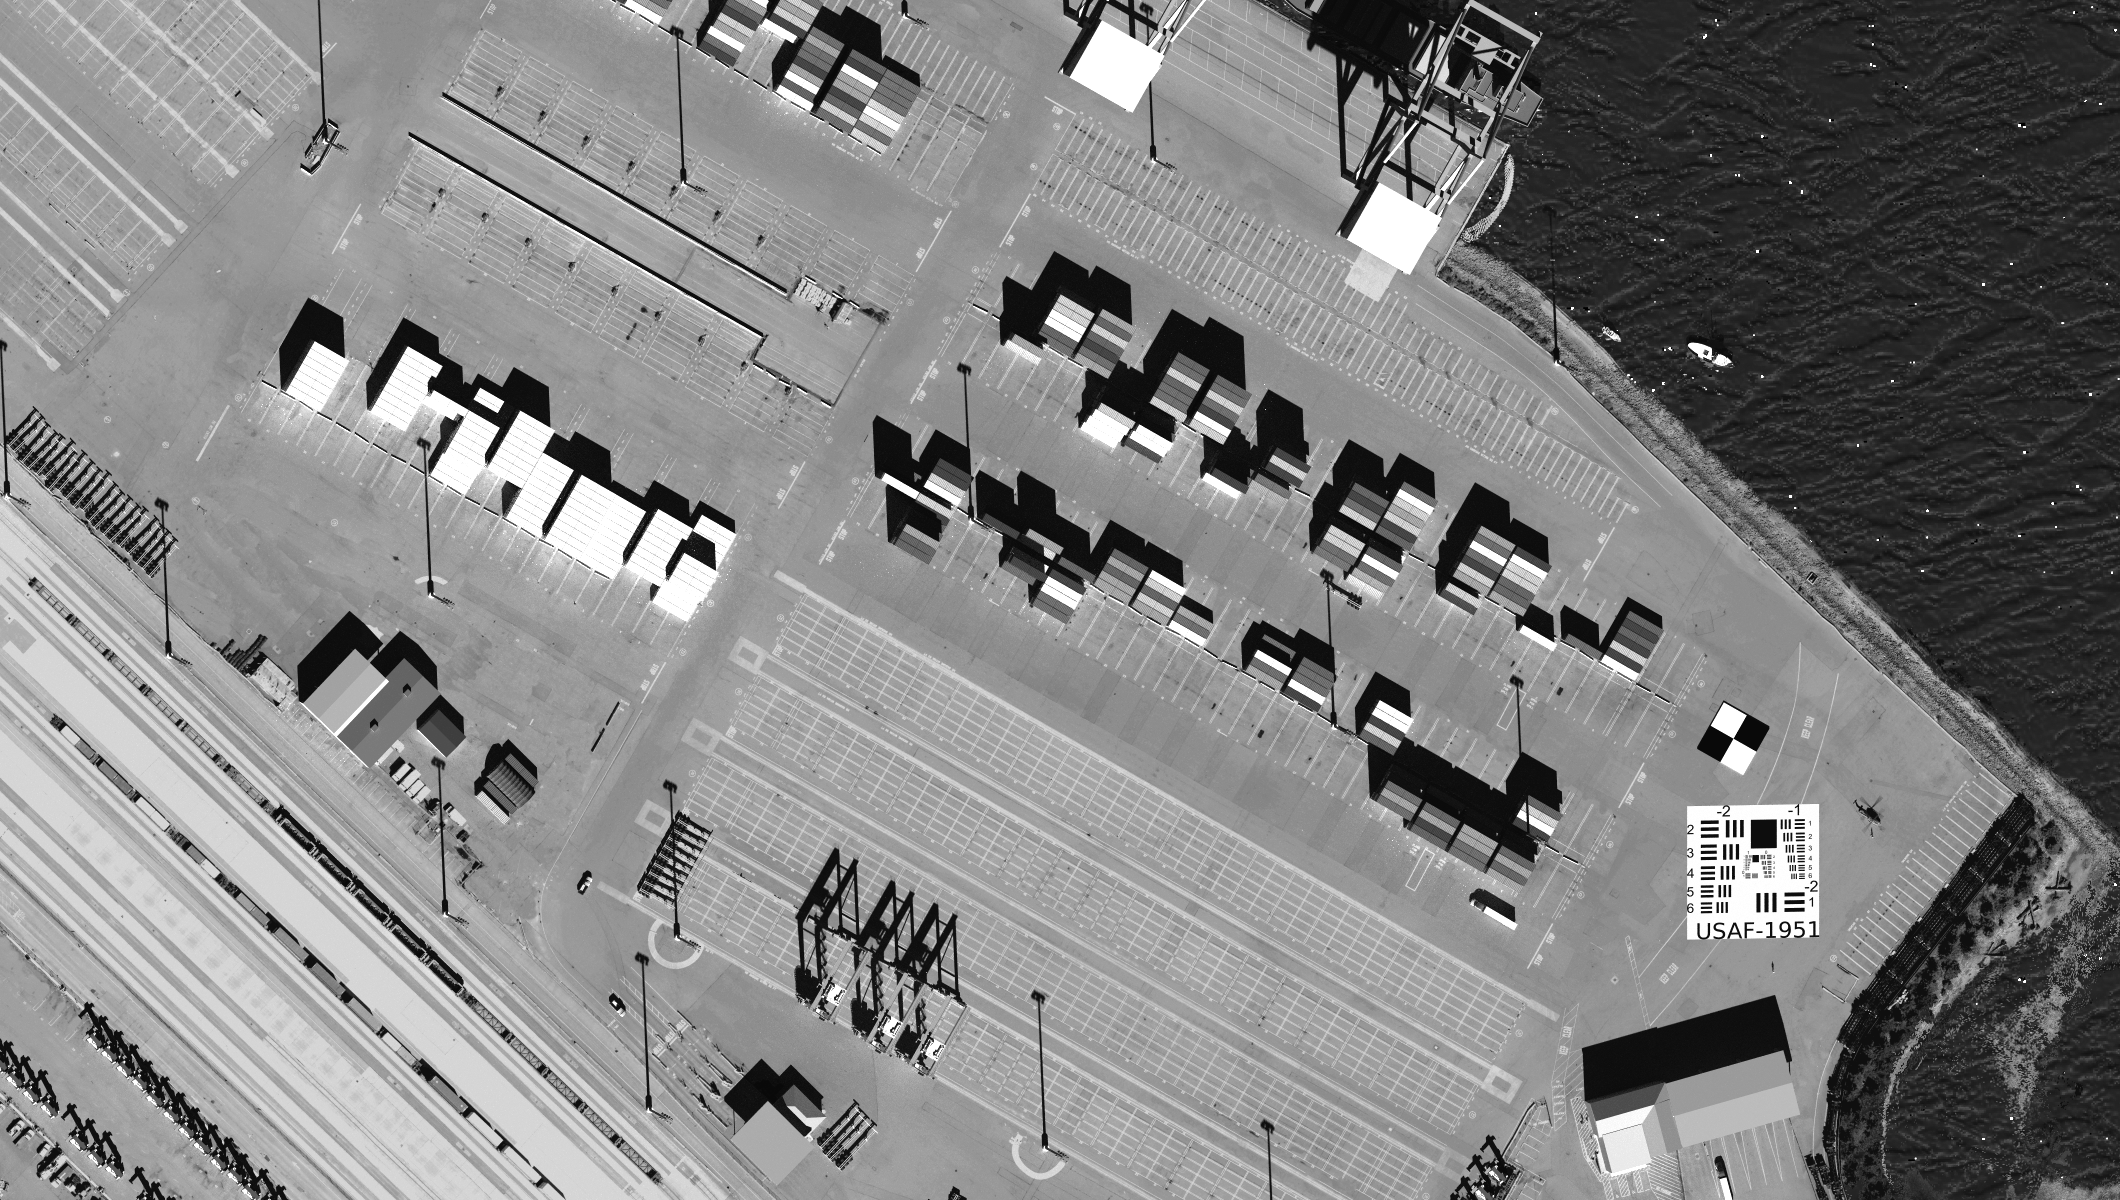
\includegraphics[width=0.49\textwidth]{tacoma}
	\caption{Frame from the Tacoma port.}
	\label{fig-tacoma}
\end{figure}

\subsection{Google Earth Engine}

Google Earth Engine is a Google project, dedicated to provide the necessary tools to analyse and visualize geospatial data. It is intended for academic studies, non-profit institutions, companies and governments. The main features of the Google Earth engine are:

\begin{itemize}
\setlength\itemsep{0em}
  \item Work with datasets from different satellites such as LANDSAT, MODIS, SENTINEL, etc.
  \item IDE to manipulate data, an extensive API that allows you to combine images from different spectral bands, see them on a world map, export data to Google Drive and more.
\end{itemize}

\section{Structure of project}
To determine the structure of the project, the different alternatives that are seen in the section \ref{estatart} are studied. Specifically, the structure of AirSim and Carla will be analysed to decide the structure of this project.

\subsection{AirSim} 
AirSim is composed of multiple modules written in various languages, as can be seen below:

\begin{itemize}
\setlength\itemsep{0em}
	\item \textbf{AirLib (C++)}: Module for Unreal Engine that provides the base classes to communicate through the RPC protocol and control the simulated vehicles.
	\item \textbf{DroneServer (C++)}: Server to receive orders from RPC client.
  	\item \textbf{DroneShell (C++)}: Shell client to send orders to the Server.
  	\item \textbf{PythonClient (Python)}: Client to send orders through RPC, it also includes code to manipulate images.
  	\item \textbf{SGM (C++)}: Code to manipulate images and generate the segmentation view.
    \item \textbf{Unity (C\# i C++)}: Unity version, includes a modules to see the AirSim information.
    \item \textbf{Unreal Engine (C++)}: Unreal version, includes a modules to see the AirSim information.
\end{itemize}

\subsection{Carla SIMULATOR}

Carla SIMULATOR is composed of multiple modules as you can see in the figure \ref{fig-carlamodules} written in multiple languages. The modules of Carla are:

\begin{figure}[h]
  	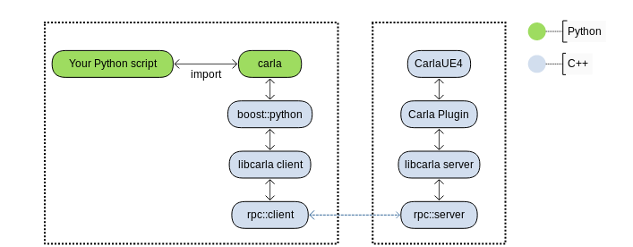
\includegraphics[width=0.49\textwidth]{carlamodules}
	\caption{Relation between the modules of Carla.}
	\label{fig-carlamodules}
\end{figure}

\begin{itemize}
\setlength\itemsep{0em}
 \item \textbf{LibCarla (C++)}: The main library of Carla, is in charge of the logic of the simulation.
 \item \textbf{Unreal (C++)}: Graphic engine with the Carla plug-in, this includes all the functionalities added to Unreal.
 \item \textbf{PythonAPI (Python)}: The API allows to send orders to the Carla module that works like a server, this API it is useful to make your own scripts.
\end{itemize}

\subsection{The structure chosen}

We have analysed two projects with similar characteristics to decide the main structure. This scheme can be seen in the figure \ref{fig-dronsimulatormodules}. A single structure has been chosen because the other projects are based on the creation of Unreal Engine assets. This factor is contrary to the purpose of this project, in which we want to load land at runtime with data which is external to the engine.

\begin{figure}[h]
\centering
  	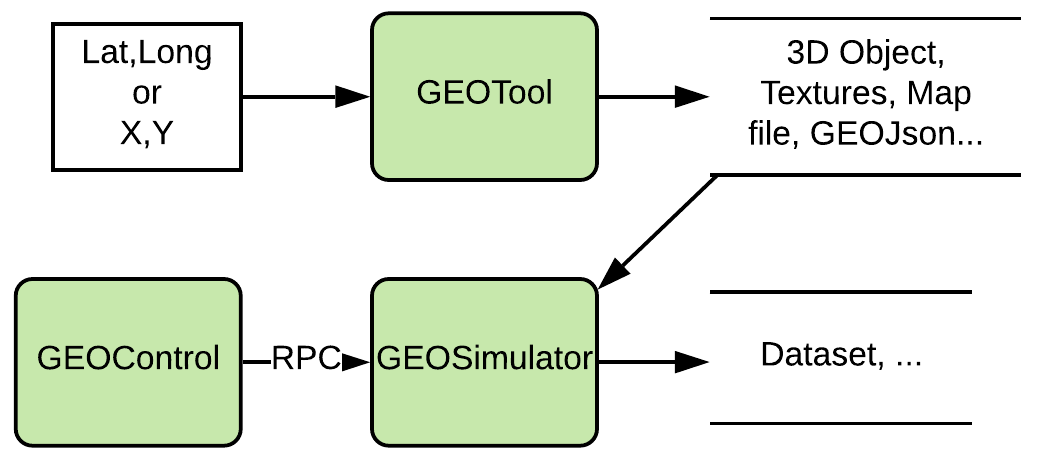
\includegraphics[width=0.45\textwidth]{structuretfg}
	\caption{Structure of GEOSpectralSimulator.}
	\label{fig-dronsimulatormodules}
\end{figure}

The project consists of the following modules:

\begin{itemize}
\setlength\itemsep{0em}
  \item \textbf{GEOTool (Python)}: The objective of GEOTool is to provide the necessary tools to obtain and transform the geographical representation in 3D representation. Base data is obtained from various sources such as: standard web services, files, etc. This module downloads and generates the necessary files to be played on a graphic engine.
  
  \item \textbf{ScriptAPI (Python)}: This module provides the necessary code to read CSV files that determine the behaviour of our vehicle. In order to do this, it’s necessary to manage time, files and the connection to the RPC client. The files control aspects such as: the position the place where you are looking from (vehicle or cameras), the possibility of obtaining an image to generate data sets and which texture you want to use.
  
  \item \textbf{Unreal Engine Simulator (C++)}: Simulator in Unreal Engine that includes the following: A library to implement the RPC server, the necessary classes to read the files generated by GEOTool and manage them, the generation of images, textures management, vehicle management and cameras, etc.
\end{itemize}

%%%%%%%%
% Module GEOTool
%%%%%%%%
\section{Module GEOTool}

In this section you can see how the GEOTool module works and what the implemented functionality is. More specifically you can see: the origin of the data, how to configure GEOTool, how the data is transformed to be read in graphics engines such as Unreal, Unity, OpenGL, etc. Finally, the generation performance will be analysed from wavefront object files (\texttt{.obj}).

\subsection{Obtaining data}
\label{getdata}

To obtain geographic data, it has been decided that the communication will use the standards proposed by the Open Geospatial Consortium \cite{ogc}: Web Map Service (WMS) \cite{wms} to obtain orthophotos and Web coverage service (WCS) \cite{wcs} to obtain maps of elevations. These services are sent as parameters to the region that you want to download. In order to carry it out, HTTP requests are used. This process is used by various institutions that follow the standard, in this case tests have been done with the ``Institut Cartogràfic i Geològic de Catalunya" \cite{icgc}.

\subsubsection{Configuration file}
\label{section:configfilegeotool}
In the configuration file (Written in JSON) we can determine: what area you want to get, what web services you want to request, etc. This file will be received by GEOTool as a command line parameter. In this file you can configure the following parameters (We can see an example with real data in the appendix \ref{appendix:geotoolconfig}):

\begin{itemize}
\setlength\itemsep{0em}
  \item \textbf{Type}: Format of the coordinates. It can be \texttt{latlng} or \texttt{xy}, in the first case, it will make the corresponding transformation to the UTM format (x, y).
  
  \item \textbf{Coordinates}: Coordinates on which we want to make the request in the format indicated in the type field. If ``xy'' is selected, the attributes x,y will be defined, and in case of choosing ``latlong" we will define the lat, long attributes.

  \item \textbf{Dimensions}: The dimension field determines the sizes that we want to download (The maximum size depends on the webservice). It is composed of:
  
  \begin{itemize}
  \setlength\itemsep{0em}
  \vspace{-0.2cm}
    \item Bbox: Bbox are the dimensions in pixels of the geographical area, this parameter is affected by ``cellsize''.
    \item Texture: Texture is a resolution in pixels request to the texture image.
  \end{itemize}
  
  \item \textbf{chunks}: The fragments that you want to download. The application calculates the displacement and generates n pieces of width$\times$height defined by BBox. It contains two parameters (height and width) to determine the number of pieces.
  \item \textbf{cellsize}: Size of each pixel in meters.
  \item \textbf{meshStep}: The number indicates the quantity of points that wish to skip on the mesh (Default: 1). More information on the section \ref{qualitat}.
  \item \textbf{Wcsurl}: The URL to the web service that will give us the height data.
  \item \textbf{folderWcs}: Folder to save the files.
  \item \textbf{Outputwcs}: Base name of the output files.
  \item \textbf{Formatwcs}: Format of the file generated by heightmaps. Available: \texttt{raw, obj} (Object 3D).
  \item \textbf{Wmsrequests}: Array with each request that will be for obtaining textures, each item is composed by:
  
  \begin{itemize}
  \setlength\itemsep{0em}
    \item Url: URL to the webservice WMS.
    \item Layers: The layers we want to get from these webservice.
    \item Name: The name of texture, used by the generated files.
    \item Format: Output format. Available: \texttt{jpg}.
  \end{itemize}
  
\end{itemize}


\subsection{Generation of terrains from a elevations maps}

In this section we explain the different options to generate files that can be read in graphics engines. It has been decided to investigate the formats: RAW and OBJ.

\subsubsection{Format RAW}

The RAW format is a format based on values of 16 bits, where the value of sea level is 128. All the heights are saved in binary format and put in a file. This format is accepted by the Unreal and Unity land builder, but has dimension limitations; You must meet several specified conditions in the Unreal Editor, this causes you to lose control of the generated mesh, the texture coordinates do not match and the texture that is applied to the mesh will have to adapt. Motivation by which it decided to add the generation of 3d objects in the standard format, generating its objects as you can see in section \ref{mesh3d}.

\subsubsection{Generation of mesh 3D}
\label{mesh3d}
To import the terrain in the graphic engine, it is decided to generate a 3D mesh in format \texttt{.obj} (format compatible with most 3D editor, graphic engine, etc.). This format offers freedom to control the distance between the vertices, the vertices where the texture is applied and the normal vectors (important for the application of lighting algorithms).
\\
\\
Because the looping is slow, all operations are performed with the NumPy library. NumPy takes advantage of the parallelism of the computer allowing to increase the speed in the calculation of matrices. The problem has been adapted to the operations of matrix type, you can see the code in the appendix \ref{appendix: generateobj}.
\\
\\
For the generation of objects four types of objects must be defined:

\begin{itemize}
\setlength\itemsep{0em}
  \item \textbf{Vertex}: They are in every vertex of the world. The vertices are identified by the index as they are inserted (1, 2, 3, ..., H $\times$ W). Each point is multiplied by a K (K represents the distance between two vertices according to the distance indicated by the elevation map obtained).

  \item {
    \textbf{Vertex of texture}: Vertex with two components x and y compressed between 0 and 1 that indicates the correspondence between the points of the texture and location in the mesh. This property is calculated with the equations \ref{equation:u} and \ref{equation:v}.
    \begin{equation}
    \label{equation:u}
    u = f(column) = column / (width - 1)
    \end{equation}
    \begin{equation}
    \label{equation:v}
    v = f(row) = 1 - (row / (height - 1))
    \end{equation}
  }

\vspace{-0.5cm}
  \item \textbf{Normal of vertex}: Vectors indicate the direction in which the light is reflected for each vertex of the object. In order to calculate these normals it is necessary to calculate the normal for each face, though these are not included in the final file because the engines generate it by default.

  \begin{itemize}
  \setlength\itemsep{0em}
    \item {
      Generation of normal faces: In order to generate the normals of a face once you know the relation between the faces, we follow the pattern you can see in the figure \ref{fig-normalpattern} where we follow the equation \ref{equation:u} for the calculation of the normal face $\vec{A}$. It makes cross product $\vec{C} = \vec{B}\times\vec{A}$ and it finally normalizes the vector $\vec{Normal} = \frac{\vec{C}}{\mid\vec{C}\mid}$.
    }

    \item {
    Generation of the normal for the vertex: In order to generate the vector normal for each vertex, we use the structure that can see in figure \ref{fig-normalpattern} applying the next equation for each vertex where V corresponds to the vertices and F corresponds to the faces on the figure \ref{fig-normalpattern}:
      \begin{equation}
      \vec{NormalV} = \vec{F_1} + \vec{F_2} + \vec{F_3} + \vec{F_4} + \vec{F_5} + \vec{F_6}
      \end{equation}
      \begin{equation}
      \vec{NormalV} = \frac{\vec{NormalV}}{\mid\vec{NormalV}\mid}
      \end{equation}
    }
  \end{itemize}

  \item \textbf{Faces}: In this step it is determined which is the union of vertices that will be used to generate the different faces of the mesh, in this implementation it is decided to make a triangulation, that is, for each square of the mesh two triangular faces are generated. It is important to generate the faces in the correct order, writing the vertices in an order opposite to the hands of the clock, in this way the graphic engine determines that the normal face will point upwards when showing the 3D mesh correctly.
\end{itemize}

\begin{figure}[h]
\centering
  	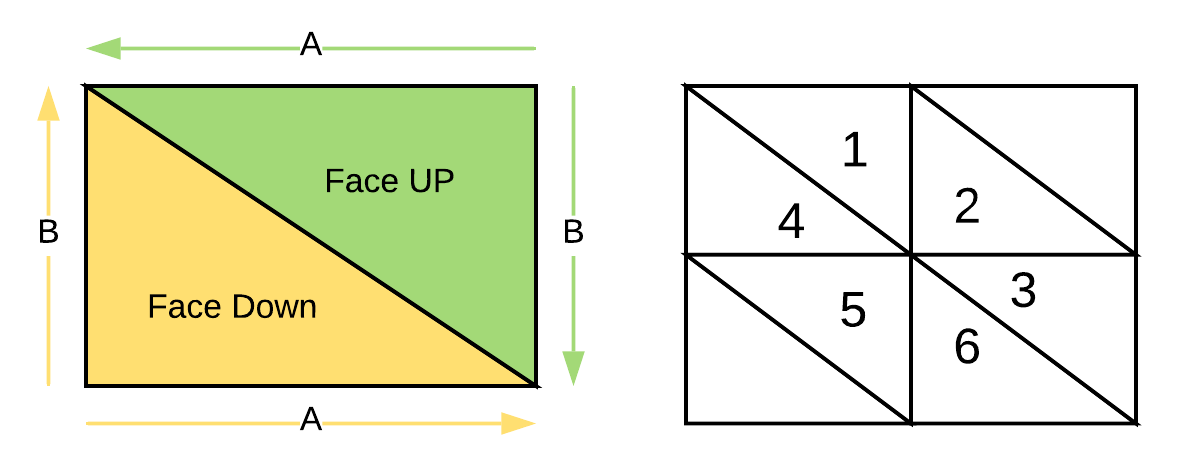
\includegraphics[width=0.49\textwidth]{patternmeshgeneration}
	\caption{Pattern for calculating the normal vector on the faces (left) and vertex (right).}
	\label{fig-normalpattern}
\end{figure}

Once the generation process has been completed, the application will generate a mesh that can be opened in any editor. You can see an example of open mesh in the MeshLabs application in the figure \ref{fig-meshlab}.

\begin{figure}[h]
\centering
  	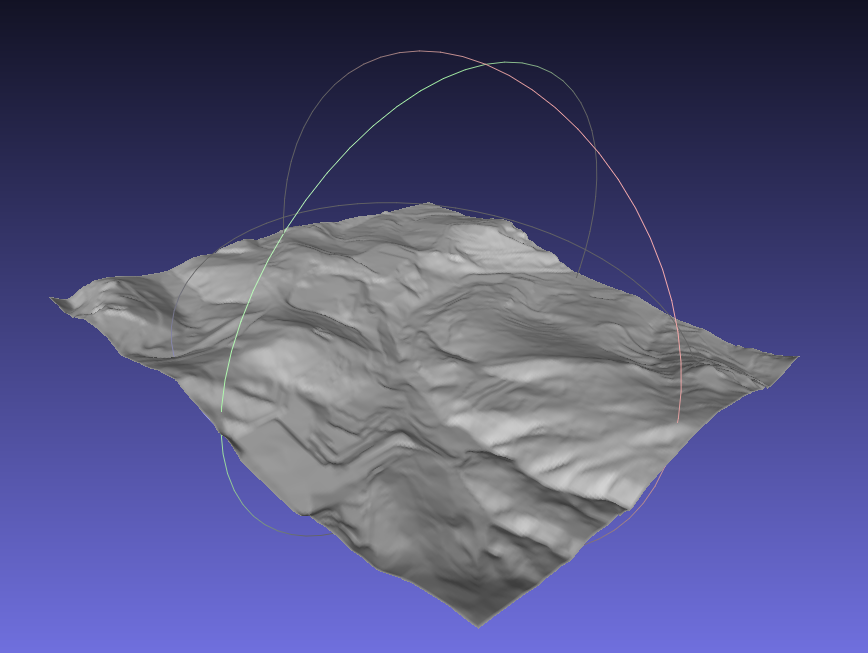
\includegraphics[width=0.49\textwidth]{mesh_example_meshlab}
	\caption{Terrain mesh visualized in software MeshLab.}
	\label{fig-meshlab}
\end{figure}

\subsubsection{GEOJson associated at the terrain}

To locate the terrain generated in third-party software that works with geospatial data, a GEOJson file is included. This file indicates which is the geographical zone that has been downloaded. An example of this can be seen in the appendix \ref{appendix:geojson}.


\subsection{Time of generation}
In this section the two versions implemented are analyzed to see the difference in generation time. This is an important point for future implementations in which the goal might be to implement a viewer in real time, where new data loads as the user moves on the world.
\\
On the figure \ref{fig-meshtime} the differences in time between the version using for loops and the version using the NumPy library can be seen. The implementation using the library NumPy is 24 times faster for a size of 500$\times$500, this is due to the fact that NumPy is optimized for parallel processing of vectorial data.

\begin{figure}[h]
\centering
  	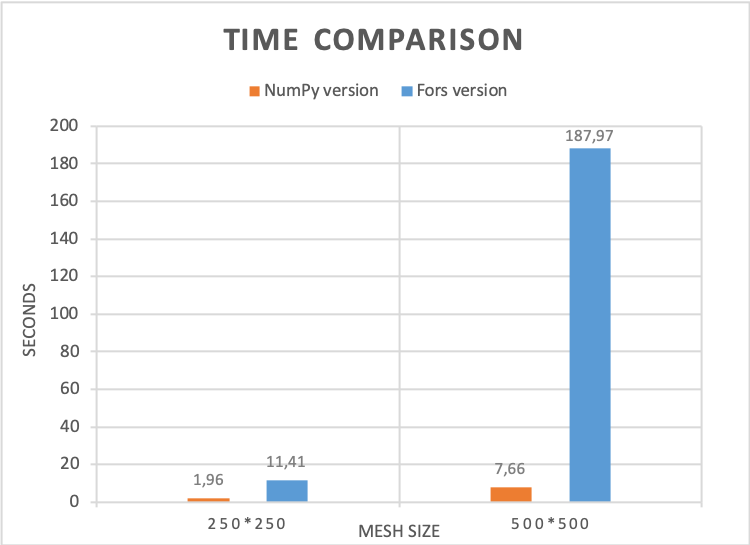
\includegraphics[width=0.4\textwidth]{meshtime}
	\caption{Graph with the time of generation of a mesh according to size.}
	\label{fig-meshtime}
\end{figure}

\subsection{Quality}
\label{qualitat}
This section shows the results of reducing the quality of the land, both qualitatively (visual difference) and quantitatively (size in bytes). To make this reduction, "meshStep" size jumps are made, established in the JSON configuration file. The tests have been carried out with powers of 2 (1,2, 4, 8, 16, ...) in the own matrix of points and using the terrain of size 300$\times$300 pixels.
\\
\\
As you can see in the figure \ref{fig-qualitatmegas} by reducing the number of points, the size in bytes is reduced exponentially, which causes the file to load faster in the Unreal environment. As you can see in the figure \ref{fig-qualityvisual}, the loss of quality is visible. If you take the mountain as a reference, you can see the loss of definition on the top of the mountain. It can be considered that visually, when ``meshStep'' is configured as 1 or 2, the loss of quality is not perceptible. At 4, you may notice a little, and finally at levels 8 and 16, you notice a noticeable loss of quality.

\begin{figure}[h]
\centering
  	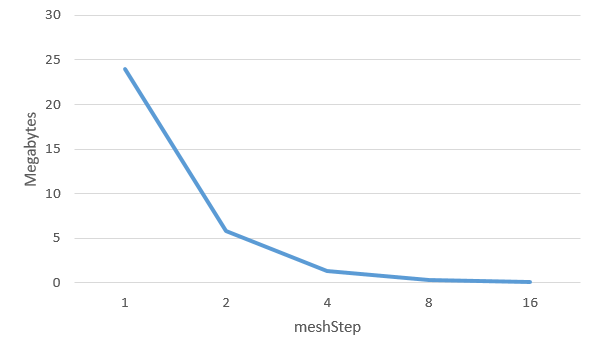
\includegraphics[width=0.4\textwidth]{qualitatmegas}
	\caption{Graph with the occupied size in bytes varying the parameter ``meshStep'' for a graph of size 300$\times$300.}
	\label{fig-qualitatmegas}
\end{figure}

\begin{figure}[h]
\centering
  	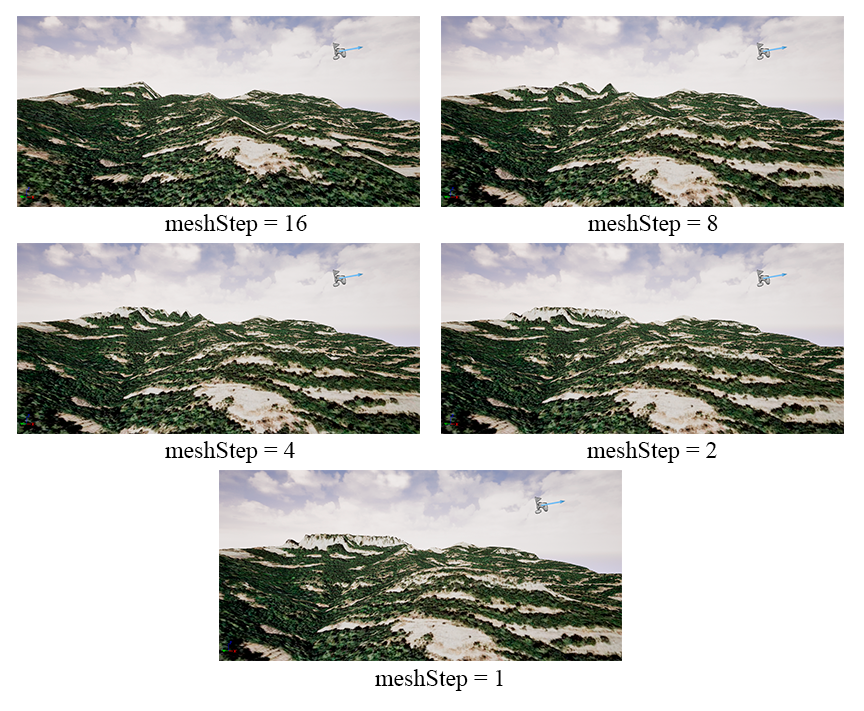
\includegraphics[width=0.49\textwidth]{quality/quality}
	\caption{Visual comparison of the effects produced by the level quality.}
	\label{fig-qualityvisual}
\end{figure}

\subsection{Map file}
 
GEOTool generates a file to be able to locate and load the scenario (map file). The map file refers to all the files downloaded with GEOTool (chunks). These parts contain basic information: location in the real world, size, size of each pixel, the textures we want to load, etc. The file follows a format so that it can be generated without using GEOTool and then loaded into the GEOSimulator module adding information of any origin (respecting the formats of the files). You can see an example in the appendix \ref{appendix:mapjson}.

%%%%%%%%
% Module Simulator
%%%%%%%%
\section{Module: Simulator}

In this section the multiple parts of which the GEOSimulator module is composed are explained. The objective of this module is to provide a tool that simulates a trip with a generic vehicle on a terrain, obtaining images of several cameras on board of the vehicle. One way to do this is to control the vehicle using the RPC protocol. In this case the RPC server is implemented in the simulator as can be seen in the section \ref{rpcserver} and it is controlled with an RPC client implemented in the GEOControl module as it can be seen in the following section \ref{modulescript}.

\subsection{Visualization and control of the vehicle}

The objective of this part is to provide the interface with the ability to move a generic vehicle in the simulated world. In the vehicle you can configure several cameras, this way you can see the same area in multiple perspectives. As an example, you can see the zenith view in the figure \ref{fig-montserratir}.

\begin{figure}[h]
\centering
  	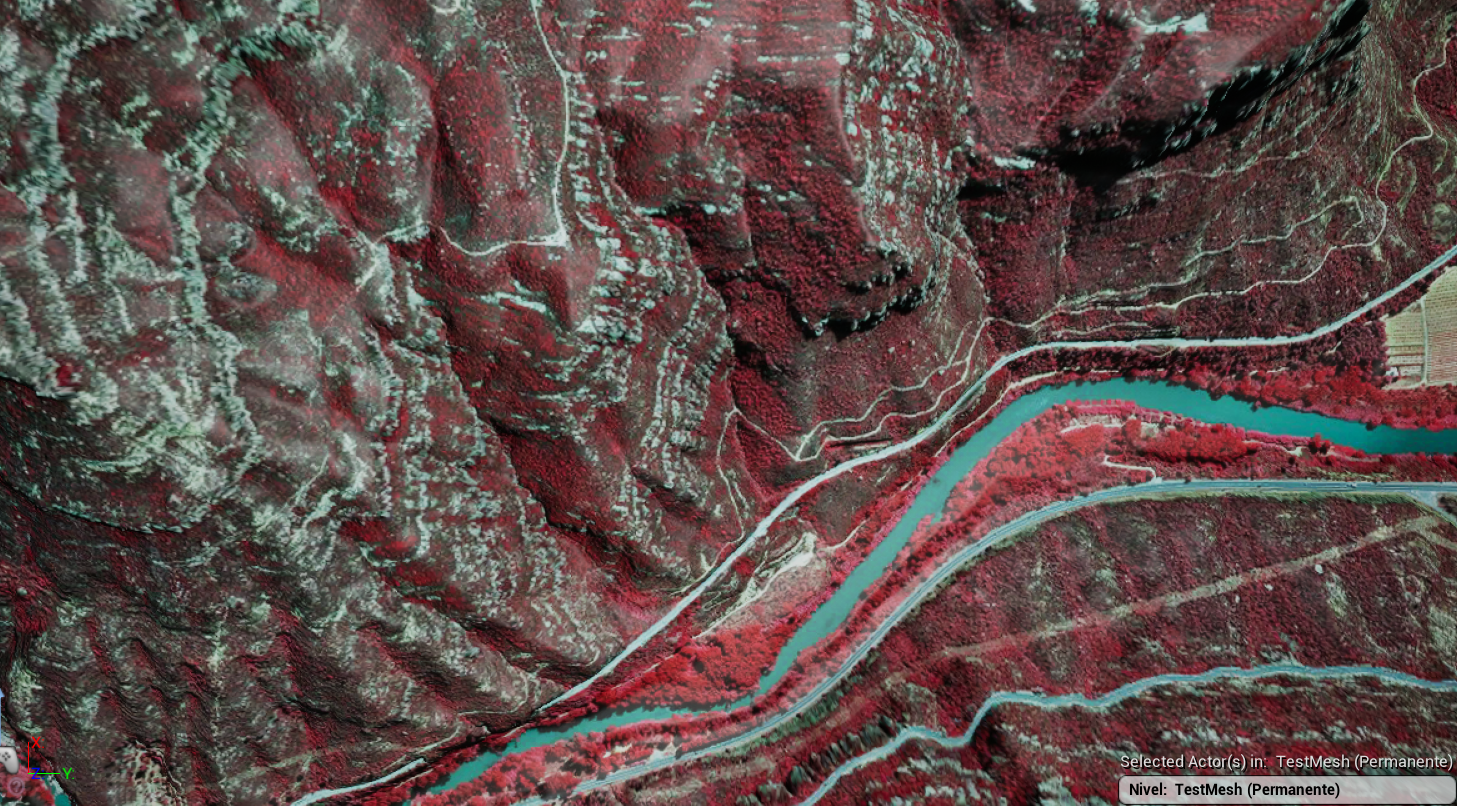
\includegraphics[width=0.49\textwidth]{cenitalviewir}
	\caption{Infrared view of Montserrat in zenith position.}
	\label{fig-montserratir}
\end{figure}

\subsubsection{Remote control}
\label{rpcserver}

In order to control the vehicle remotely, a communication using the RPC protocol (Remote Procedure Call) is implemented. More specifically, it is by using the Rpclib \cite{rpclib} library for C++. This server is implemented in the GEOSimulator module. The administration of the RPC server is done through an ``AVehiclePawn'' class. This class can be inherited so that we can add more specific functionality (vehicles of different types, specific behaviours, etc.). The following actions are implemented: initialize / stop the RPC server, change the position of the vehicle, change the rotation of the vehicle or cameras (implemented with Look At), request images of one of the cameras that will be generated, etc.
\\
The assignment of the functions is done in the function \texttt{void BindFunctions(rpc::server* server)} that the server instance receives. This function can be overwritten to add more functionality (To see how to do it see the appendix \ref{appendix:extendrpc}). By default, the ``AVehiclePawn'' class allows us to call the following RPC functions:


\begin{itemize}
\setlength\itemsep{0em}
\item \texttt{setLocation(double x, double y, double z)}: Send the location on which one place the vehicle.

\item \texttt{setLookAt(double x, double y, double z)}: Send a vector with the position in the world you want to look at, from which point the simulator should keep the camera's eyes.

\item \texttt{setLocationAndLookAt(double x, double y, double z, double lx, double ly, double lz)}: The function that implements the two previous calls in a single call.

\item \texttt{setCameraLookAt(int cameraId, double x, double y, double z)}: A function that chooses a camera and configures in what direction the camera looks at.

\item \texttt{getImage(int idCamera, std::string path, std::string channel)}: Generates images using the following information: the camera that will generate the image, the place where the image are going to be saved and the texture from which you want to obtain the image. All this is done synchronously, to guarantee that the image is generated in the correct position.
\end{itemize}

\subsubsection{Sky visualization}

To implement the sky, the native Unreal module is used, where a sphere is generated in which the sky is represented. It has multiple parameters to configure the sky in multiple ways, some of the things that can be done are: determine the position of the sun, the lighting of the stars, the amount of clouds, the speed of the clouds, etc.
\\\\
This allows to generate synthetic images at different times of the day with different lighting to generate more complex data sets. On the other hand, if you want to get the maximum realism you have to use textures without shadows causing Unreal to generate them, otherwise it will create an undesired effect. An example of the different hours of the day can be seen in the figure \ref{fig-sky}.

\begin{figure}[h]
\centering
  	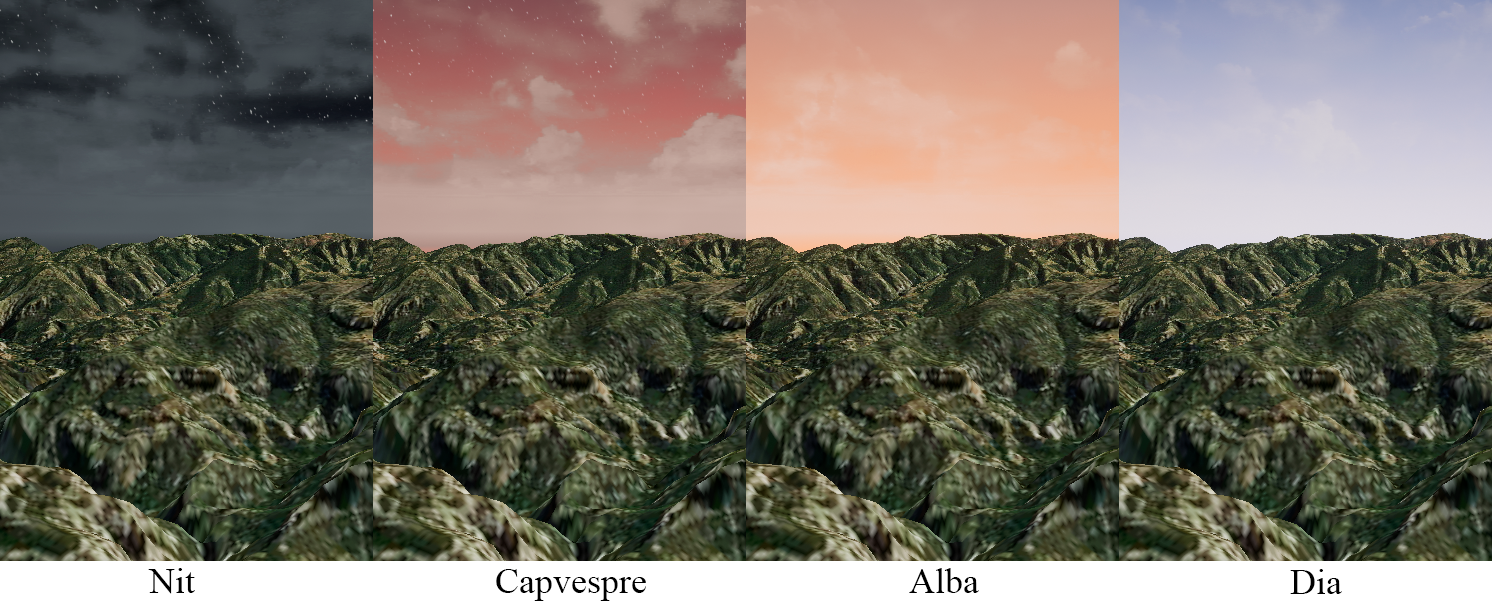
\includegraphics[width=0.49\textwidth]{sky/sky}
	\caption{Example of differents sky.}
	\label{fig-sky}
\end{figure}

\subsection{Terrain}
The terrain is loaded through the code executed at runtime, for it loads the \texttt{obj} file and is processed using the class UProceduralMesh \cite{uprocedural}, this class allows us to add the geometrical information to the simulator. To load the meshes, it must be considered that Unreal works with a different system of coordinates, in which the y axis is inverted with respect to the UTM model. Due to this, it is necessary to make the necessary changes.
\\
\\
This mesh is loaded in the world and it is represented by the class ``MapChunk'', this class is assigned a dynamic material that allows to change between the loaded textures. The texture can be any image prepared to be used as a texture in Unreal, giving the possibility to see RGB, infrared, multispectral bands, indices generated by multispectral data, etc.

\begin{figure*}[h]
\centering
    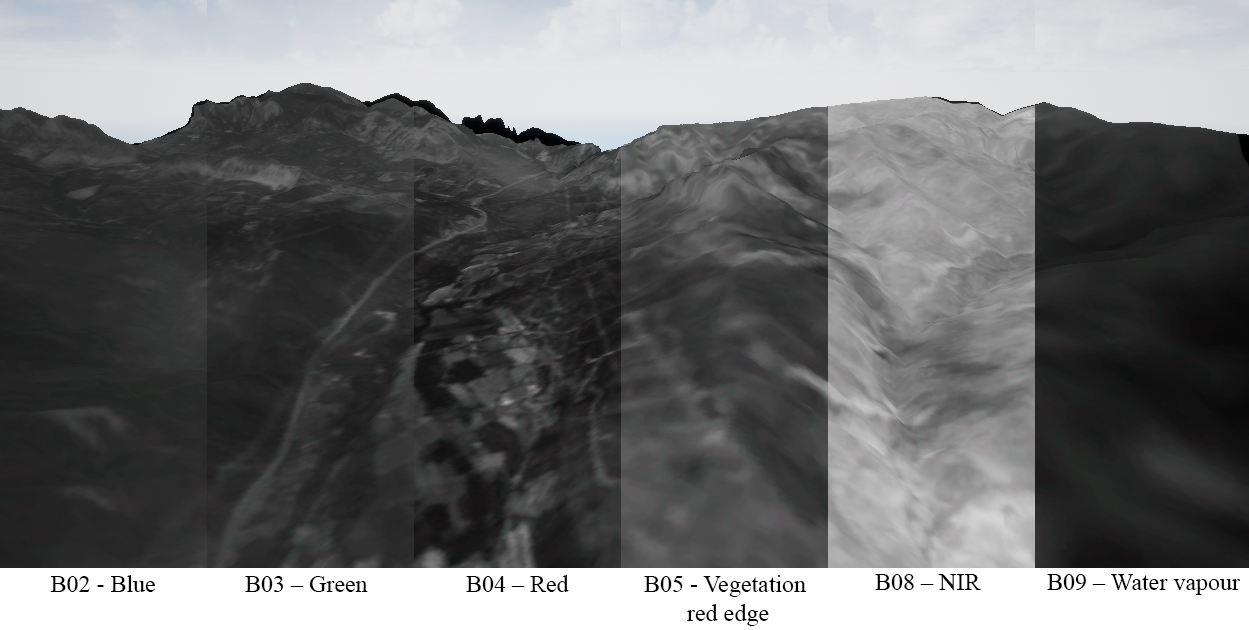
\includegraphics[width=1\textwidth]{multispectral/bands}
  \caption{View of ''Sales de Pallars'' in six different spectral bands.}
  \label{fig-bands}
\end{figure*}

\begin{figure*}[h]
\centering
  	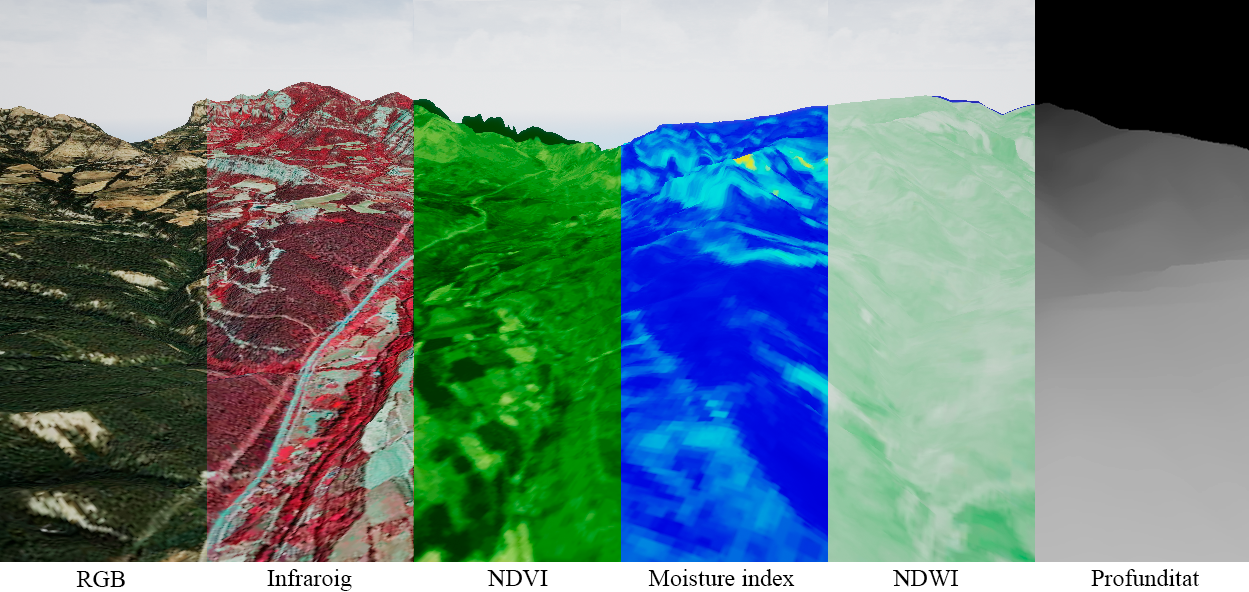
\includegraphics[width=1\textwidth]{multispectral/spectralindexes}
	\caption{View of ``Sales de Pallars'' in RGB, infrared, NDVI, moisture, NDWI and depth.}
	\label{fig-spectralindexes}
\end{figure*}

\subsection{Results of visualization of terrains}
In this section you can see the results obtained from visualizing 3D generated by the GEOTool module in the GEOSimulator module. To generate these results, images from different sources have been used, more specifically, the RGB and infrared views are obtained from the ``Institut Cartogràfic de Catalunya'', the multispectral data is obtained from the Sentinel 2 \cite{sentinel2} satellite through the EO Browser \cite{eobrowser} and depth data are generated by applying a shader to the camera.
\\
\\

You can see in Figure \ref{fig-bands} how it has been applied to a terrain that corresponds to ``Sales de Pallars'', different multispectral bands obtained from the satellite Sentinel 2. The first three bands B02, B03 and B04 correspond to the bands of colours, the band B05 corresponds to the fast change of the reflectance that is produced in the vegetation in a range near the infrared, the band B08 obtains NIR \cite{nir} data and the B09 is able to detect water vapours.

With these bands composed data from multiple spectrums that can be applied to multiple scopes is obtained. In figure \ref{fig-spectralindexes} some examples can be seen, between them the indexes are:

\begin{itemize}
\setlength\itemsep{0em}
\item 
{
	NVDI \cite{ndvi}: Based on the combination of the bands (B08 - B04)/(B08 + B04), index used to see the farming state.
}
\item
{
	Moisture index \cite{moisture}: Based on the combination of the bands (B8A - B11)/(B8A + B11), indicates the proportion of precipitation that is needed to satisfy the needs of vegetation.
}
\item
{
	NDWI \cite{ndwi}: Based on the combination of the bands (B03 - B08)/(B03 + B08), the index is used to determine the hydrique stress of the vegetation, saturation of the humidity in the land or limit the mass of water in lakes or reservoirs.
}
\end{itemize} 

The last view of the figure \ref{fig-spectralindexes} the depth or proximity can be seen using  algorithms of 3D reconstruction with monocular stereo, prevention of collisions, algorithm of multiview stereo, etc.

\subsection{How to interact with the simulator}
In order to interact with the simulator the following keys have been defined:

\begin{itemize}
\setlength\itemsep{0em}
\item A,W,S,D: Left, Front, Back, Right movement of the vehicle.
\item Alt, SpaceBar: Down and up the vehicle.
\item Q,E: Left and right rotation of vehicle.
\item Y: Starts an RPC Server
\item U: Stops an RPC Server.
\item H: Show/Hide the visualization of vehicle.
\item K: Save image in the simulator folder from the second camera.
\end{itemize}

%%%%%%%%
% Module Scripting
%%%%%%%%
\section{Scripting module}
\label{modulescript}

This section contains an explanation of the main points of the scripting module. Some of the functionalities of this module are: read trajectory files, read control files of cameras, manage time, request images, etc.

\subsection{Paths}
The scripting module allows you to make trips, read trajectories created in a real world (adapting this to the correct format) or generate synthetic trajectories. In this way, a trajectory that has been previously made can be recreated in the simulator, it can be reproduced as many times as desired. This allows us to carry out multiple tests with different visualizations of the land passing through the same points. For this, finally, some files are generated in CSV format that are explained in the section \ref{file-trajectories}.

\subsubsection{File of paths}
\label{file-trajectories}
Now it's explained how to configure the path file and the file to place the cameras. The file is in CSV format and can be read from the GEOControl module to indicate to the simulator the positions of the vehicle and where both the vehicle and the cameras should be viewed (in UTM coordinates).

The file which controls the vehicle is composed by the next fields:

\begin{itemize}
\setlength\itemsep{0em}
\item Time: Time in milliseconds from start of the script.
\item x, y, z: Position X, Y, Z in UTM format.
\item LookX, LookY, LookZ: Position X, Y, Z to which we look in UTM format.
\end{itemize}

The file which controls the cameras is in another file composed of the fields:

\begin{itemize}
\setlength\itemsep{0em}
\item Time: Time in milliseconds from start of the script.
\item cameraId: The Id of the camera that want to modify.
\item LookX, LookY, LookZ: Position X, Y, Z to which we look in UTM format.
\item GetImage: Boolean (0 or 1) that indicates if you want to generate an image from this camera in this instant of time.
\item Channel: Textures of which we want to obtain images separated by \textbar.
\end{itemize}

An example from the CSV file generated with Excel can be seen in the appendix \ref{appendix:fitxerscsv}.

\subsection{Noise simulation}

Vehicles experience sudden movements due to wind, asphalt conditions and other factors. To simulate this, noise has been introduced in the trajectory of the tests. During the first’s tests, noise was generated through code, but that way the tests can't be reproduced multiple times. Due to that, that strategy was dismissed. After that, the noise was introduced directly in the CSV files pertaining to the trajectory. This option is better because it allows to work with external files produced by real vehicles, drones or synthetic which guarantees that the tests can be reproduced multiple times.

\subsection{Generation of Datasets}
One of the objectives of this project is to offer the possibility of generating data sets of synthetic images generated by the simulator. In order to generate data sets, the ``GetImage'' field is used, as seen in the section \ref{trajectory-file}, which generates an image each time it finds this field in 1.

In the figure \ref{fig-dataset} there is a little example with a few images of a tour on which the camera its fixed with a concrete point that it is left behind with the passage of time.

\begin{figure}[h]
\centering
  	\includegraphics[width=0.49\textwidth]{dataset/dataset}
	\caption{Set of images generated by GEOControl.}
	\label{fig-dataset}
\end{figure}

\section{Full workflow to generate a dataset}

This section shows an example of the workflow that can be achieved with the modules generated in this project. This will show you how to use them and will serve to think about new applications that can be developed using this project as a base.
\\
\\
First, the GeoTool module is used to obtain data: For this we will obtain the coordinates of the area we want to obtain, we can use applications such as Google Maps. In this case it is used to download the area of the ``Santa Margarita Volcano'', the approximate coordinates (lat 42.130596, longitude 2.521956) are selected to obtain the area around it. Once chosen, the JSON is configured, which can be seen in the section \ref{section:configfilegeotool}. Once the process is completed, the module is called with the following command: \texttt{./GEOTool.sh config.json} (the requirements to execute this application can be seen in the appendix \ref{appendix:requirementsgeotool}). Once the process is finished, a series of files are generated, as can be seen in the figure \ref{fig-filesgeotool}.

\begin{figure}[h]
\centering
  	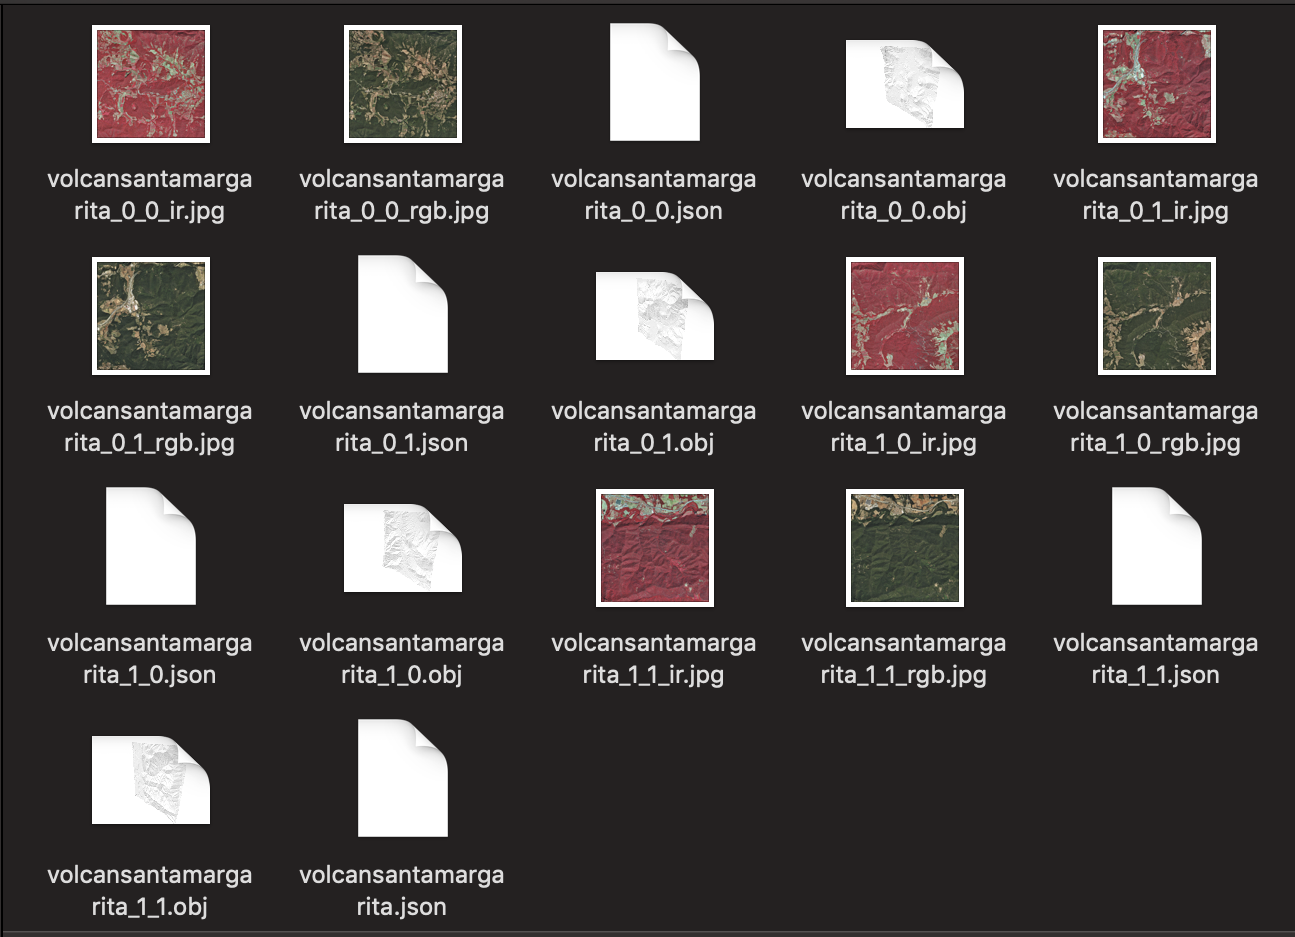
\includegraphics[width=0.49\textwidth]{filesgeotool}
	\caption{Files generated by GEOTool.}
	\label{fig-filesgeotool}
\end{figure}

Once the map is generated, the files will be added to the folder ``Maps'' which is located next to the simulator's executable. The simulator will run with the following command \texttt{./GEOSimulator.sh -folderMap="Maps/volcan/" -map="volcan.json"}. Once the simulator has been initialized, it can be seen in the interface located in the upper left corner: the position in the world where the vehicle is located and the status of the RCP server, an example can be seen in the figure \ref{fig-workflowsimulator}.

The RPC server can be initialized with the Y key, and once this is done, the module that controls the vehicle and requests the generation of images will be invoked.

\begin{figure}[h]
\centering
  	\includegraphics[width=0.49\textwidth]{simulatorworkflow}
	\caption{Simulator view.}
	\label{fig-workflowsimulator}
\end{figure}

With the files containing the trajectories already created as indicated in the section \ref{file-trajectories}, the GEOControl module can be invoked with the following command \texttt{./GEOControl.sh filevehicle.csv filecamera.csv} (the requirements to run this application can be seen in the appendix \ref{appendix:requirementsgeocontrol}). This module will execute and generate the data set in the folder of ``output''. You can see an example in the figure \ref{fig-dataset}.

\section{Conclusions}

This project shows how to obtain textures and elevation maps originated from satellites, this information can be manipulated to generate indexes, new information generated through neural networks, etc. The processed data is transformed into 3D information that can be interpreted by graphics engines such as Unreal Engine. It has taken into account aspects such as the time needed to generate the 3D model, which have been analysed to see the effect of libraries like NumPy during matrix manipulation, accelerating the process thanks to parallelism. You get faster times thanks to the reduction of points to generate 3D models, this reduction is useful for rendering large models.

The section pertaining to the simulation module shows the information in a 3D enviroment generated with Unreal Engine. We can add cameras to a simulated vehicle and see different perspectives of the same information. To do this, another module has been created, which sends commands to an RPC server implemented in Unreal Engine, in which we can move, choose where the vehicle looks in the real world, where cameras point to and obtain the images captured by the cameras.
The tests, which were performed with data from Satellites like the Sentinel 2, show how this information is represented in the simulated environment, which use has each type of data and what possibilities the simulator offers when seeing this information.

The section pertaining to the scripting shows how to generate trajectories that can be reproduced multiple times in the simulated enviroment, which allows to make several journeys with different data, or the same journey observing this data from multiple perspectives, extracting this information in the form of datasets. These trajectories can control multiple parameters of the vehicle and in which point and from which cameras the images are obtained. In the real world, the vehicle experiences unexpected movements due to several factors, like wind and the conditon of the asphalt. To simulate this, a filter that generates noise has been added, to induce random movements to the vehicle and the camera.

\section*{Acknowledgments}

First of all, I want to thank  my tutor Felip Lumbreras for the time he invested in this project, the help provided when consulting experts and all the ideas provided during meetings. Secondly, I would like to thank Marc Garcia for guiding me in the use of Unreal Engine and helping me complete this project successfully. Thirdly, I would like to thank my friends Javier García Cantero and Jordi Miranda for helping me by revising the English version of this paper. And lastly, I would like to thanks the project BOSSS TIN2017-89723-P.

\begin{thebibliography}{11}
\bibitem{agile}
Agile software development
\\ \url{https://en.wikipedia.org/wiki/Agile_software_development}
[19/02/2019]
 
\bibitem{kanban}
Kanban
\\ \url{https://www.iebschool.com/blog/metodologia-kanban-agile-scrum/} [19/02/2019]

\bibitem{trello}
Trello - \url{https://trello.com/} [19/02/2019]

\bibitem{airsim}
AirSim - \url{https://github.com/Microsoft/AirSim} [19/02/2019]

\bibitem{carla}
Carla SIMULATOR - \url{http://carla.org} [19/02/2019]

\bibitem{less}
LESS - \url{http://lessrt.org/} [11/04/2019]

\bibitem{dirsig}
Digital Imaging and Remote Sensing Image Generation - \url{http://dirsig.org/} [11/04/2019]

\bibitem{googleearth}
Google Earth Engine - \url{https://earthengine.google.com/} [20/05/2019]

\bibitem{unreal}
Unreal Engine - \url{https://www.unrealengine.com/en-US/what-is-unreal-engine-4} [09/03/2019]

\bibitem{ogc}
Open Geospatial Consortium (OGC) -  \url{http://www.opengeospatial.org/} [08/04/2019]

\bibitem{wms}
Web Map Service (WMS) -  \url{https://www.opengeospatial.org/standards/wms} [08/04/2019]

\bibitem{wcs}
Web Coverage Service (WCS) -  \url{https://www.opengeospatial.org/standards/wcs} [08/04/2019]

\bibitem{icgc}
Institut Cartogràfic i Geològic de Catalunya (ICGC) - \url{http://www.icgc.cat/ca/} [08/04/2019]

\bibitem{wavefrontobj}
Wavefront .obj file - \url{https://en.wikipedia.org/wiki/Wavefront_.obj_file} [09/04/2019]

\bibitem{rpclib}
RPC Lib - Modern mgspack-rpc for C++ - \url{http://rpclib.net/} [10/04/2019]

\bibitem{uprocedural}
Procedural Mesh Component - \url{https://wiki.unrealengine.com/Procedural_Mesh_Component_in_C%2B%2B:Getting_Started} [21/05/2019]

\bibitem{eobrowser}
EO Browser - \url{https://apps.sentinel-hub.com/eo-browser/} [25/05/2019]

\bibitem{sentinel2}
Sentinel 2 - \url{https://www.esa.int/esl/ESA_in_your_country/Spain/SENTINEL_2} [25/05/2019]

\bibitem{nir}
Tecnología NIR, sus Usos y Aplicaciones - \url{https://www.engormix.com/balanceados/articulos/tecnologia-nir-sus-usos-t32534.htm} [25/05/2019]

\bibitem{ndvi}
El NDVI o Índice de vegetación de diferencia normalizada - \url{https://geoinnova.org/blog-territorio/ndvi-indice-vegetacion/} [25/05/2019]

\bibitem{moisture}
Moisture index - \url{http://glossary.ametsoc.org/wiki/Moisture_index} [25/05/2019]

\bibitem{ndwi}
Cálculo del índice NDWI - \url{http://www.gisandbeers.com/calculo-del-indice-ndwi-diferencial-de-agua-normalizado/} [25/05/2019]

\end{thebibliography}

\newpage
\appendix
\section*{Appendix}

\setcounter{section}{1}

\subsection{List of objectives}
\label{appendix:objectives}
\begin{enumerate}
  \item Analyze.
  \item Define a structure.
  \item Developing.
  \begin{enumerate}
    \item Develop module GEOTool.
    \begin{enumerate}
		\item Develop configuration file.
		\item Develop the transformation to RAW and OBJ.
		\item Develop reduction of quality.
		\item Develop map file.
  	\end{enumerate}
  	
    \item Develop module GEOSimulator
    \begin{enumerate}
	  	\item Develop vehicle logic
	  	\item Develop RPC Server
	  	\item Develop the image acquisition
	  	\item Develop movement of cameras
  	\end{enumerate}
  	
  	\item Develop module GEOControl
	 \begin{enumerate}
	  	\item Develop clock for all scripts
	  	\item Develop csv files.
  	\end{enumerate}  	
  	
  \end{enumerate}
  
  \item Test
  \item Keep record
\end{enumerate}

\subsection{JSON example for configure GEOTool}
\label{appendix:geotoolconfig}
\lstinputlisting{geotoolconfig.json}

\subsection{Code for generate a 3D mesh from a heights file}
\label{appendix:generateobj}
\lstinputlisting[language=Python]{generateobj.py}

\subsection{GEOJson example}
\label{appendix:geojson}
\lstinputlisting{geojson.json}

\subsection{Map file generated by GEOTool}
\label{appendix:mapjson}

Example of JSON with 2 chunks.
\lstinputlisting{mapjson.json}

\subsection{Example code for understand the RPC functionality}
\label{appendix:extendrpc}

\lstset{language=C} 
\begin{lstlisting}
.h:
	virtual void BindFunctions(rpc::server* server) override;
	
.cpp:
void MyClass::BindFunctions(rpc::server* server)
{
	Super::BindFunctions(server);

	server->bind("nameOfFunction", [context_params](Variables...) {
		//MyCode
	});
}

\end{lstlisting}

\subsection{Example of CSV file to control the vehicle and cameras}
\label{appendix:fitxerscsv}

\vspace{0cm}
\begin{figure}[!h]
\centering
  	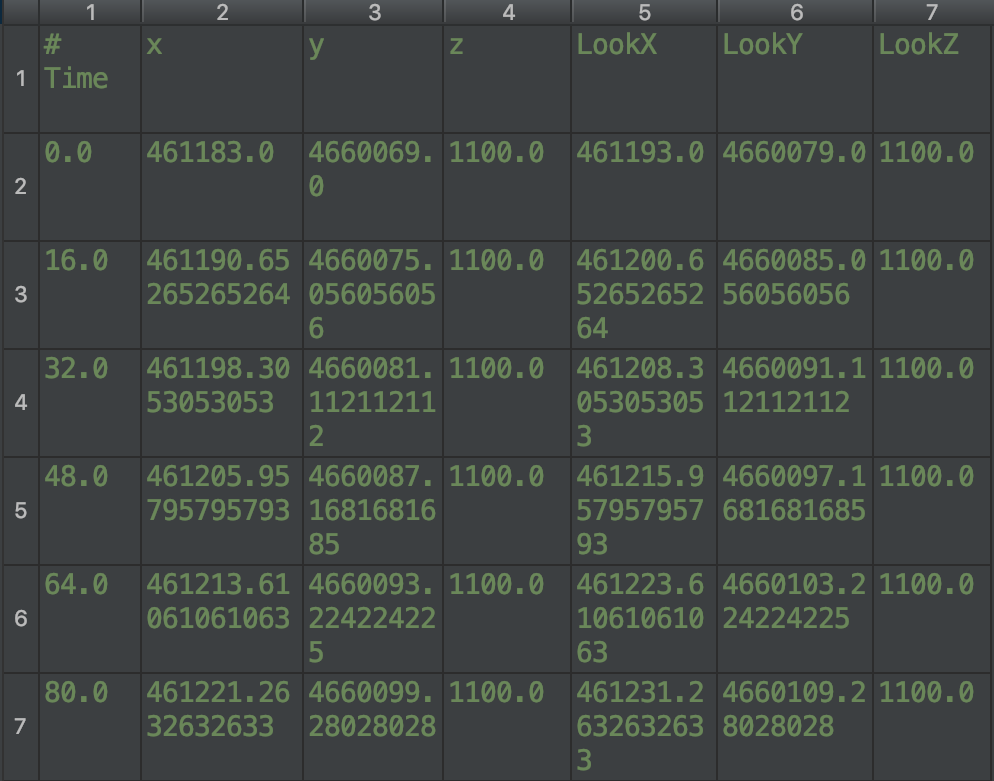
\includegraphics[width=0.45\textwidth]{fitxervehicle}
	\captionsetup{labelformat=empty}
	\caption{CSV file to control a vehicle}
	\label{fig-fitxervehicle}
\end{figure}

\vspace{0cm}
\begin{figure}[!h]
\centering
  	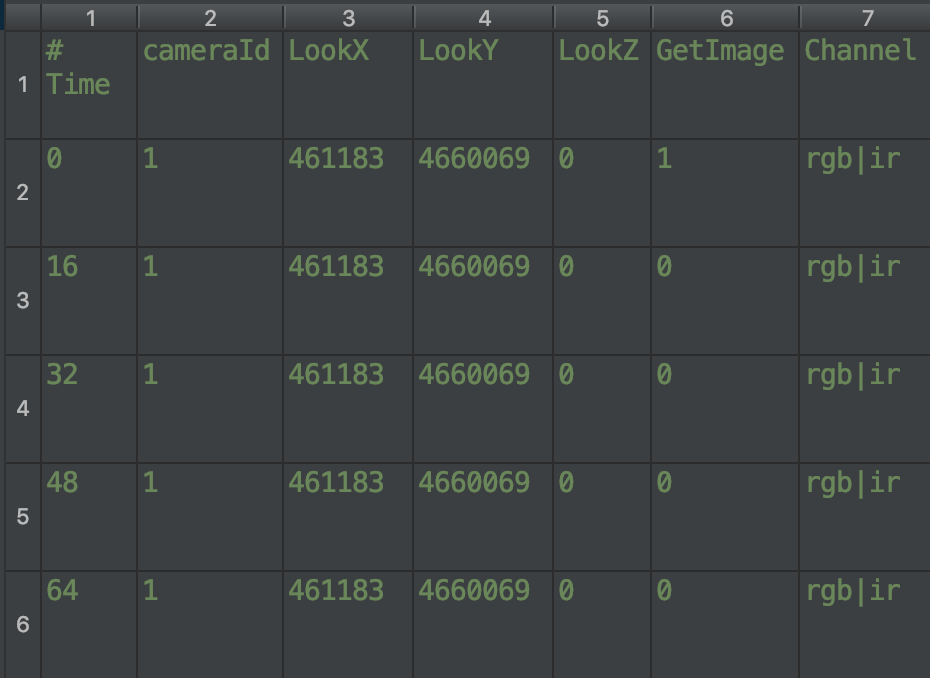
\includegraphics[width=0.45\textwidth]{fitxercameres}
  	\captionsetup{labelformat=empty}
	\caption{CSV file to control cameras}
	\label{fig-fitxercameres}
\end{figure}

\subsection{Requirements to execute GEOTool}
\label{appendix:requirementsgeotool}

In order to use this application correctly we will have to have installed the Anaconda package (Tested with version 4.6.11 and Python 3.7.3) to which the 'utm' library will be installed with the command ''pip install utm''.

\subsection{Requirements to execute GEOControl}
\label{appendix:requirementsgeocontrol}

In order to use this application correctly we will have to have installed the Anaconda package (Tested with version 4.6.11 and Python 3.7.3) to which the ''mprpc'' library will be installed with the command ''pip install mprpc''.


\end{document}

